
\documentclass{beamer}	
\mode<presentation>
 
\usepackage{pdfpages}
\usepackage{fancyvrb}
\usepackage{chemarr}

\usepackage{amsmath}		%% mathematics typesetting
\usepackage{amssymb}
 
\usepackage{epigraph}   %% nice setting of quotations

\usepackage{tabularx} %% allows to use row colours in tables

\usepackage{ulem}

\usepackage{booktabs}

\usepackage{siunitx} %% tpyeset SI units

\usepackage{CJKutf8} %% typeset Chinese characters

\usepackage{pdfpages}%% include pdfs

\usepackage{graphicx}
\usepackage{animate} %% show animated gifs

\DeclareMathAlphabet{\mathcalligra}{T1}{calligra}{m}{n}


% Color and Theme. Can be changed. However, this one's quite nice.
\usetheme{Madrid}
\definecolor{theme}{rgb}{0.84,0,0.21}
\usecolortheme[named=theme]{structure}

%%  Title information
\title[M01.9 Repetitorium Physik]{M01.9 Repetitorium Physik \\ Teil 2}
\author[melanie.stefan@medicalschool-berlin.de]{}
\institute[]{Prof. Ervice Pouokam Kamgne, Prof. Melanie Stefan \\ melanie.stefan@medcialschool-berlin.de}
\date{SoSe 2022}
 

% Table of contents to pop up at the beginning of each section
\AtBeginSection[]
{
  \begin{frame}<beamer>
    \frametitle{Outline}
    \tableofcontents[currentsection,currentsubsection]
  \end{frame}
}
 
\beamertemplatenavigationsymbolsempty

\begin{document}


{ \usebackgroundtemplate{
\includegraphics[width=1.2\paperwidth]{MSB_Titelseite.pdf}} 
\begin{frame}

 \maketitle 

$\,$\\[6cm] 
\end{frame}
}

\section{M01.1 Methodik, Grundbegriffe, Fehlerrechnung}

%% Rechnen allgemein

% % Basiseinheiten und häufige abgeleitete Einheiten des SI-Systems benennen
% %  Vektoren, Skalare, Exponentialfunktionen, Logarithmen, Trigonometrischen Funktionen, Integration und Differentialrechnung erklären
%     %  Dezimale Vielfache von Einheiten sprachlich und durch Zehnerpotenzen darstellen
%     % mit Funktionsgraphen arbeiten
% % erkennen, warum Physik in der Medizin wichtig ist
% %  rechnen ohne Angst


% \begin{frame}{Rechnen}
    


% \begin{columns}[c]
% \begin{column}{5cm}

% % frequently used einheiten
% \begin{block}{SI Einheiten}
% \begin{center}
%     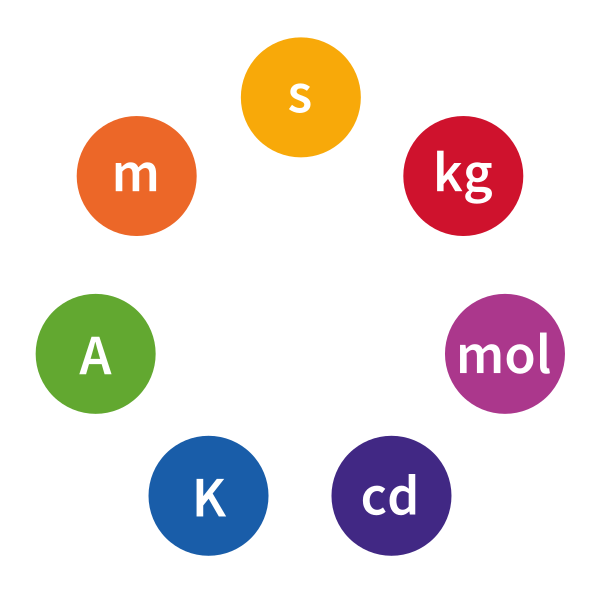
\includegraphics[width=\textwidth]{SI_base_units.png}
% \end{center}


% (Alles andere ist abgeleitet)
% \end{block}


% %% frequently used zehnerpotenzen
% \begin{block}{Zehnerpotenzen}

% \begin{tabular}{ll|ll}
% dezi (d)        &   \(10^{-1}\) & deka      & \(10^{1}\)    \\
% zenti (c)       &  \(10^{-2}\)  & hekto (h) & \(10^{2}\)    \\
% milli (m)       & \(10^{-3}\)   & kilo  (k) & \(10^{3}\)    \\
% mikro (\(\mu\)  & \(10^{-6}\)   & mega  (M) & \(10^{6}\)    \\
% nano (n)        & \(10^{-9}\)   & giga  (G) & \(10^{9}\)    \\
% pico (p)        & \(10^{-12}\)  & tera  (T) & \(10^{12}\)   \\

% \end{tabular}

% \end{block}

% \end{column}

% \begin{column}{5cm}

% %% Frequently used rechnungen

% %% Frequenty used numbers

% \end{column}

% \end{columns}

    
% \end{frame}


%% Fehlerrechnung

\begin{frame}{Messunsicherheit}

    % Messunsicherheit erklären
%  mit Messgrößen rechnen
%  Messunsicherheit darstellen und abschätzen
    
\end{frame}


%% Stats
\begin{frame}{Statistik}

% Mittelwert, Standardabweichung, und Standardabweichung des Mittelwerts erklären 
% Eigenschaften der Gaußschen Glockenkurve benennen
%  Mittelwert, Standardabweichung, und Standardabweichung des Mittelwerts berechnen
% verstehen, warum manche Konzepte (Gaußsche Glockenkurve, Logarithmen, Differential etc.) oft vorkommen

    
\end{frame}



%% Methodik IMPP Fragen


% %% Würfel
\begin{frame}{IMPP-Fragen zu M01.1}

\textbf{Würfelförmige Zellen mit jeweils \(10\,\mu m\) Kantenlänge  bilden mit vernachlässigbar kleinen Zwischenräumen ein Gewebe.}

\textbf{Wie viele Zellen sind in \(1\,cm^3 \) eines derartigen Gewebes enthalten?}

\begin{decription}
\item[A]
1000
\item[B]
1 Million
\item[C]
1 Milliarde
\item[D]
100 Milliarden
\item[E]
1 Billion
\end{decription}

    
\end{frame}

\begin{frame}{IMPP-Fragen zu M01.1}

\textbf{Würfelförmige Zellen mit jeweils \(10\,\mu m\) Kantenlänge  bilden mit vernachlässigbar kleinen Zwischenräumen ein Gewebe.}

\textbf{Wie viele Zellen sind in \(1\,cm^3 \) eines derartigen Gewebes enthalten?}


Wie viele Zellen pro Kante? 



\begin{columns}[c]


\begin{column}{5cm}
%% pictures from iphone



\end{column}


\begin{column}{5cm}
%% pictures from iphone


\[1\,cm = 10^{-2}\,m\]

\[10\,\mu m = 10^{-5}\,m\]

\[

\frac{10^{-2}}{10^{-5}} = 10^{-2-(-5)} = 10^3
 
\]


\end{column}



\end{columns}

    
\end{frame}






% \begin{frame}{IMPP-Fragen zu M01.1}
    
% \end{frame}


% %% Messfehler

% Die Messunsicherheit eines Blutdruckmessgeräts wird in der Bedienungsanleitung mit \(\pm 3\, mmHg\) angegeben. Bei einer Messung wird als diastolischer Wert \(90\,mmHg\) angezeigt.

% Etwa wie groß ist somit die relative Mssunsicherheit dieses Wertes (wenn die Angabe in der Bedieungsanleitung zutrifft)?


% \begin{decription}
% \item[A]
% \(\pm 0,2\,\%\) 
% \item[B]
% \(\pm 0,3\,\%\) 
% \item[C] 
% \(\pm 0,9\,\% \) 
% \item[D]
% \(\pm 2\,\%\) 
% \item[E]
% \(\pm 3\,\%\) 
% \end{decription}

% \begin{frame}{IMPP-Fragen zu M01.1}
    
% \end{frame}


% %% Männer

% Bei einer großen Anzahl männlicher Probanden wurde eine Reihenuntersuchung durchgeführt. Es ergab sich für die Körpergröße eine (Gauß-) Normalverteiling mit einem Mittelwert von \(1,80\,m\) und einer Standardabwichung von \(10\,cm\) 

% Welche Aussage zur Größenverteilung dieser Männer trifft am ehesten zu? 
% \begin{decription}
% \item[A]
% Etwa \(5\,\%\) sind mindestens \(2\,m\) groß
% \item[B]
% Etwa \(16\,\%\) sind höchstens \(1,50 \, m\) groß
% \item[C] 
% Etwa \(32\,\% \) sind zwischen \(1,70\,m\) und \(1,90\,m\) groß

% \item[D]
% Etwa \(50\,\%\) sind mindestens \(1,80\,m\) groß
% \item[E]
% Etwa  \(68\,\%\) sind höchstens \(1,90\,m\) groß
% \end{decription}





%% Irgendwas mit Fehlern?


\section{M01.2 Mechanik}

\section{M01.3 Aerodynamik Hydrodynamik, Viskosität und Grenzflächeneffekte}


\section{M01.5 Schwingungen und Wellen}





%% %% %% %% Feedbackhinweisblock

% \begin{frame}
% \frametitle{Danke für Ihr Feedback!}

% \begin{columns}[c]

% \begin{column}{6cm}
% \begin{center}
%  \includegraphics[width=\textwidth]{smilie_balloons.jpg}
% \end{center}

% \end{column}

% \begin{column}{4cm}


% \begin{center}
% \includegraphics[width=\textwidth]{feedback_QR.png}
% \end{center}
% \end{column}


% \end{columns}
% \end{frame}


%% %% %% Bildnachweis
\begin{frame}
\frametitle{Bildnachweis}
\begin{tiny}

\begin{itemize}



\item
SI Einheiten. User:DePiep, CC BY-SA 3.0 \url{https://creativecommons.org/licenses/by-sa/3.0}, via Wikimedia Commons
% %%%%%%%%%%%



\end{itemize}
\end{tiny}
\end{frame}






\end{document}

%%% Frequently used snippets

%% \begin{columns}[c]

%% \begin{column}{5cm}
%% \end{column}

%% \begin{column}{5cm}
%% \end{column}


%% \end{columns}




